\documentclass{beamer}

\usepackage{../cppenv}
\usepackage{../recdefs}

\usetheme{Rochester}
\usecolortheme{crane}

\usepackage{pifont}
\newcommand{\tick}{\ding{51}}
\newcommand{\cross}{\ding{55}}
\newcommand{\done}{\rlap{\(\square\)}{\raisebox{2pt}{\large\hspace{1pt}\tick}}\hspace{-2.5pt}}

\usepackage{hyperref}

\title{CS100 Recitation 11}
\author{GKxx}
\date{May 2, 2022}

\AtBeginSubsection{
    \begin{frame}{Contents}
        \tableofcontents[currentsection, currentsubsection]
    \end{frame}
}

\begin{document}

\begin{frame}
    \maketitle
\end{frame}

\begin{frame}{Contents}
    \tableofcontents
\end{frame}

\section{Overview: A Federation of Languages}

\begin{frame}{What have we learnt?}
    \begin{center}
        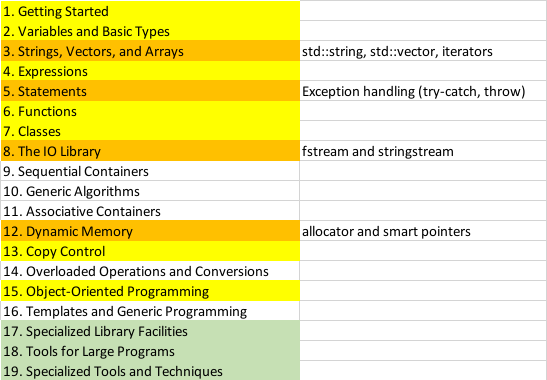
\includegraphics[width=0.95\textwidth]{img/contents.png}
    \end{center}
\end{frame}

\begin{frame}{A Federation of 4 Languages}
    \textit{Effective C++} Item 1: View C++ as a federation of languages.
    \begin{itemize}
        \item[\done] C
        \item[\done] Object-Oriented C++
        \item[\(\square\)] Template C++
        \item[\(\square\)] The STL
    \end{itemize}
\end{frame}

\section{Operator Overloading: First Glance}

\begin{frame}{Operator Overloading}
    \begin{itemize}
        \item At least one class-type parameter.
        \item Cannot change the \textbf{precedence} or the \textbf{associativity}.
    \end{itemize}
    Operators that may be overloaded:
    \begin{center}
        \begin{tabular}{|cccccc|}
            \hline
            \ttt{+} & \ttt{-} & \ttt{*} & \ttt{/} & \ttt{\%} & \ttt{\^{}}\\
            \ttt{\&} & \ttt{|} & \ttt{\~} & \ttt{!} & \redtt{,} & \ttt{=}\\
            \ttt{<} & \ttt{>} & \ttt{<=} & \ttt{>=} & \ttt{++} & \ttt{--}\\
            \ttt{<<} & \ttt{>>} & \ttt{==} & \ttt{!=} & \redtt{\&\&} & \redtt{||}\\
            \ttt{+=} & \ttt{-=} & \ttt{/=} & \ttt{\%=} & \ttt{\^{}=} & \ttt{\&=}\\
            \ttt{|=} & \ttt{*=} & \ttt{<<=} & \ttt{>>=} & \ttt{[]} & \ttt{()}\\
            \ttt{->} & \ttt{->*} & \ttt{new} & \ttt{new[]} & \ttt{delete} & \ttt{delete[]}\\
            \hline
        \end{tabular}
    \end{center}
\end{frame}

\begin{frame}{Operator Overloading}
    Operators that may not be overloaded:
    \begin{center}
        \begin{tabular}{|cccc|}
            \hline
            \ttt{::} & \ttt{.} & \ttt{.*} & \ttt{?:}\\
            \hline
        \end{tabular}
    \end{center}
    Overloaded operator is a function:
    \begin{itemize}
        \item A special name: the \bluett{operator} keyword followed by the symbol of the operator.
        \item Non-member function: Operands are the parameters from left to right.
        \item Member function: The leftmost operand is implicitly bound to \bluett{this}. Other operands are the parameters from left to right.
    \end{itemize}
    \pause
    \textit{More Effective C++} Item 7 says that \blue{never overload operator \ttt{\&\&}, \ttt{||} and \ttt{,}}. Why?
\end{frame}

\begin{frame}{Operator Overloading}
    We have seen that
    \begin{itemize}
        \item The IO library overloads \bluett{operator<<} and \bluett{operator>>}.
        \item The string library overloads \bluett{operator+} and \bluett{operator[]}.
        \begin{itemize}
            \item Why won't `\ttt{"ABC" + "DEF"}' compile?
        \end{itemize}
    \end{itemize}
\end{frame}

\section{The IO Library}

\subsection{\ttt{<iostream>}}

\begin{frame}[fragile]{\ttt{iostream}, \ttt{cin} and \ttt{cout}}
    \begin{itemize}
        \item \ttt{std::cin}: object of type \ttt{std::istream}.
        \item \ttt{std::cout}: object of type \ttt{std::ostream}.
        \item \ttt{std::istream} and \ttt{std::ostream} are \textbf{uncopyable} types.
        \pause
        \item Outputs can be chained together as in `\ttt{cout << a << b}'. Why?
    \end{itemize}
    \pause
    \begin{cpp}
inline std::ostream &operator<<
        (std::ostream &os, const Point2d &p) {
  os << "(" << p.get_x() << ", " << p.get_y() << ")";
  return os;
}
    \end{cpp}
\end{frame}

\begin{frame}[fragile]{Test the State of \ttt{iostream}}
    On input failure, no error would be thrown, but we can test this by using the stream object as a condition.
    \begin{cpp}
struct Vector2d {
  double x, y, norm_l2;
};
inline std::istream &operator>>
        (std::istream &is, Vector2d &v) {
  is >> v.x >> v.y;
  // On input failure, set the object to a valid state.
  if (is)
    v.norm_l2 = std::sqrt(v.x * v.x + v.y * v.y);
  else
    v = Vector2d{};
  return is;
}
    \end{cpp}
\end{frame}

\begin{frame}[fragile]{Examples}
    Read an unknown number of integers?
    \begin{cpp}
std::vector<int> v;
int x;
while (std::cin >> x)
  v.push_back(x);
    \end{cpp}
    \pause
    Read a line as a string?
    \begin{cpp}
std::string line;
std::getline(std::cin, line);
    \end{cpp}
    \pause
    \begin{itemize}
        \item \ttt{std::getline} reads until the first newline character (`\textbackslash n'), and throws away that newline character.
        \item What happens?
        \begin{cpp}
int n; std::cin >> n;
std::string line;
std::getline(std::cin, line);
        \end{cpp}
    \end{itemize}
\end{frame}

\begin{frame}[fragile]{Manipulators}
    \ttt{endl}, \ttt{flush} and the like are \textbf{manipulators}.
    \begin{itemize}
        \item \ttt{endl} outputs a newline character and flushes the buffer.
        \item \ttt{flush} only flushes the buffer.
    \end{itemize}
    More manipulators: (some defined in \ttt{<iomanip>})
    \begin{itemize}
        \item \ttt{boolalpha}, \ttt{noboolalpha}
        \item \ttt{oct}, \ttt{hex}, \ttt{dec}, \ttt{showbase}, \ttt{noshowbase}, \ttt{setbase}
        \item \ttt{fixed}, \ttt{setprecision}, \ttt{scientific}
        \item \dots\dots
    \end{itemize}
    \textit{C++ Primer} 17.5
\end{frame}

\subsection{\ttt{<fstream>}}

\begin{frame}[fragile]{File Streams}
    Read an unknown number of integers from a file `\ttt{student\_score.txt}'?
    \begin{cpp}
std::ifstream infile("student_score.txt");
// Equivalent way:
// std::ifstream infile;
// infile.open("student_score.txt");
std::vector<int> score;
int x;
while (infile >> x)
  score.push_back(x);
infile.close();
    \end{cpp}
\end{frame}

\begin{frame}{Inheritance}
    \begin{columns}
        \begin{column}{0.6\textwidth}
            \begin{center}
                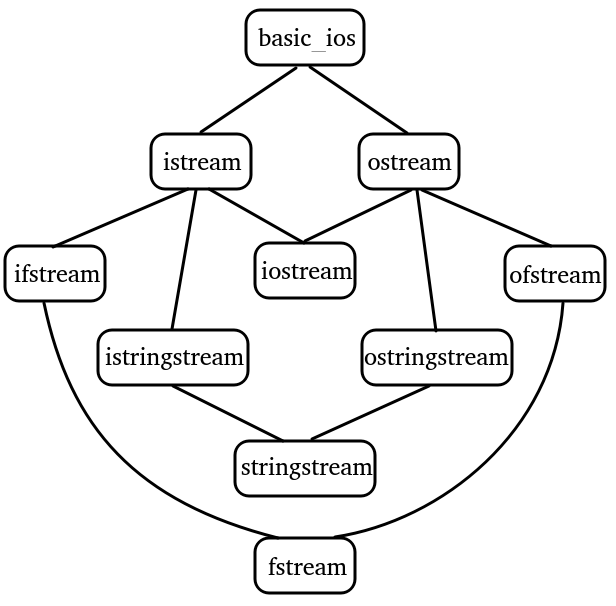
\includegraphics[scale=0.425]{img/iostream_inheritance.png}
            \end{center}
        \end{column}
        \begin{column}{0.4\textwidth}
            \begin{itemize}
                \item Multiple inheritance
                \item Virtual inheritance
                \item What can we know from this?
            \end{itemize}
        \end{column}
    \end{columns}
\end{frame}

\begin{frame}[fragile]{Real World Example}
    Read a `\ttt{.tex}' file. Change math from `\$\dots\$' to `\textbackslash(\dots\textbackslash)'.
    \begin{cpp}
std::ifstream infile("hw3.tex");
std::ofstream result("result.tex");
bool in_math = false;
std::string line;
while (std::getline(infile, line)) {
  // process the line
}
infile.close();
result.close();
    \end{cpp}
\end{frame}

\begin{frame}[fragile]{File Modes}
    Append something to a file, instead of overwriting it?
    \begin{cpp}
std::ofstream out_file("name.txt", std::ofstream::app);
    \end{cpp}
    \pause
    \begin{center}
        \begin{tabular}{|ll|}
            \hline
            \ttt{in} & Open for input\\
            \ttt{out} & Open for output\\
            \ttt{app} & Seek to the end before every write\\
            \ttt{ate} & Seek to the end immediately after the open\\
            \ttt{trunc} & Truncate the file\\
            \ttt{binary} & Do IO operations in binary mode\\
            \hline
        \end{tabular}
    \end{center}
    \begin{itemize}
        \item \textit{C++ Primer} 8.2.2
    \end{itemize}
\end{frame}

\subsection{\ttt{<sstream>}}

\begin{frame}[fragile]{Stringstreams}
    Read data from a string, or generate a string by writing different kinds of data.
    \begin{cpp}
struct Person_info {
  std::string name;
  std::vector<std::string> phones;
};
std::string line;
std::vector<Person_info> people;
while (std::getline(std::cin, line)) {
  Person_info info;
  std::istringstream record(line);
  record >> info.name;
  std::string phone;
  while (record >> phone)
    info.phones.push_back(phone);
  people.push_back(info);
}
    \end{cpp}
\end{frame}

\begin{frame}[fragile]{Stringstreams}
    Convert some \bluett{double} or \bluett{int} to a string?
    \begin{cpp}
inline std::string convert(double value) {
  std::ostringstream oss;
  oss << value;
  return oss.str();
}
    \end{cpp}
    \pause
    It works, but \ttt{std::to\_string} is a better choice!
\end{frame}

% Sequential containers
\section{\ttt{string}, \ttt{vector} and Iterators}

\subsection{\ttt{std::string}}

\begin{frame}[fragile]{Construction}
    \begin{center}
        \begin{tabular}{|ll|}
            \hline
            \begin{cpp}
string s1;
            \end{cpp} & Default initialization. \ttt{s1} contains \ttt{""}.\\
            \begin{cpp}
string s2(s1);
            \end{cpp} & Copy initialization. \ttt{s2} is a copy of \ttt{s1}.\\
            \begin{cpp}
string s2 = s1;
            \end{cpp} & Equivalent to \ttt{string s2(s1)}.\\
            \begin{cpp}
string s3("hello");
            \end{cpp} & \ttt{s3} is a copy of the string literal.\\
            \begin{cpp}
string s3 = "hello";
            \end{cpp} & Equivalent to \ttt{string s3("hello")}.\\
            \begin{cpp}
string s4(n, c);
            \end{cpp} & Initialize \ttt{s4} with \ttt{n} copies of a \bluett{char }\ttt{c}.\\
            \hline
        \end{tabular}
    \end{center}
    \begin{itemize}
        \item A string object is \textbf{NOT} null-terminated!
    \end{itemize}
\end{frame}

\begin{frame}[fragile]{IO}
    \begin{center}
        \begin{tabular}{|ll|}
            \hline
            \begin{cpp}
os << s
            \end{cpp} & Writes \ttt{s} onto output stream \ttt{os}.\\
            \begin{cpp}
is >> s
            \end{cpp} & Reads a string from \ttt{is} into \ttt{s}.\\
            \begin{cpp}
getline(is, s)
            \end{cpp} & Reads a line of input from \ttt{is} into \ttt{s}.\\
            \hline
        \end{tabular}
    \end{center}
    \begin{itemize}
        \item \ttt{is >> s} starts reading \textbf{from the first non-whitespace character}, and reads until the next whitespace character. The whitespace in the end \textbf{is not read and still in the stream}.
        \item \ttt{getline(is, s)} starts reading \textbf{from the next character} and reads until the first newline character. The newline character is \textbf{read, but not stored into \ttt{s}, and thrown away}.
    \end{itemize}
\end{frame}

\begin{frame}[fragile]{Operations}
    \begin{center}
        \begin{tabular}{|ll|}
            \hline
            \begin{cpp}
s.empty()
            \end{cpp} & \footnotesize Returns \bluett{true} iff \ttt{s} is empty (\ttt{""}).\\
            \begin{cpp}
s.size()
            \end{cpp} & \footnotesize Returns the number of characters in \ttt{s}.\\
            \begin{cpp}
s[n]
            \end{cpp} & \footnotesize Returns a \textbf{reference} to the character indexed \ttt{n} in \ttt{s}.\\
            \begin{cpp}
s1 + s2
            \end{cpp} & \footnotesize Returns a \ttt{string} that is the concatenation of \ttt{s1} and \ttt{s2}.\\
            \begin{cpp}
s1 = s2
            \end{cpp} & \footnotesize Copy-assignment. Replaces the content in \ttt{s1} with a \textbf{copy} of \ttt{s2}.\\
            \begin{cpp}
s1 += s2
            \end{cpp} & \footnotesize Equivalent \red{(?)} to \ttt{s1 = s1 + s2}.\\
            \begin{cpp}
==,!=
            \end{cpp} & \footnotesize Equality and inequality.\\
            \begin{cpp}
<,<=,>,>=
            \end{cpp} & \footnotesize Lexicographical-order comparison.\\
            \hline
        \end{tabular}
    \end{center}
\end{frame}

\begin{frame}[fragile]{Operations}
    Concatenation: \ttt{s1 + s2}.
    \begin{itemize}
        \item \ttt{s1} and \ttt{s2} can be a C-style string (\const\bluett{char }\ttt{*}) or a \bluett{char}.
        \item At least one of \ttt{s1} and \ttt{s2} should be \ttt{std::string}!
        \item \ttt{s + "a" + "b"} compiles, while \ttt{"a" + "b" + s} does not compile. Why?
    \end{itemize}
\end{frame}

\begin{frame}[fragile]{Operations}
    \ttt{s1 += s2} and \ttt{s1 = s1 + s2} are \textbf{NOT} actually equivalent:
    \begin{cpp}
auto n = 1000000;
std::string s = "";
for (auto i = 0; i != n; ++i)
  s += "a";
s = "";
for (auto i = 0; i != n; ++i)
  s = s + "a";
    \end{cpp}
    The first loop takes \(O(n)\) time, while the second takes \(O\left(n^2\right)\)!
    \begin{itemize}
        \item Always prefer compound assignment operators.
    \end{itemize}
\end{frame}

\begin{frame}[fragile]{Operations}
    \ttt{s.size()} returns a value of the type \ttt{std::string::size\_type}.
    \begin{itemize}
        \item An unsigned integer type.
        \item It is guaranteed to be able to store the length of any string.
        \item It is highly possible that it is \ttt{std::size\_t}, but not guaranteed.
    \end{itemize}
    \pause
    \ttt{s.length()} is equivalent to \ttt{s.size()}, but \ttt{s.size()} is preferred. \red{(Why?)}
\end{frame}

\begin{frame}[fragile]{Examples}
    Example: Convert a nonnegative integer to a string. Add leading zeros.
    \begin{cpp}
inline std::string convert(int x) {
  auto s = std::to_string(x);
  return std::string(9 - s.size(), '0') + s;
}
    \end{cpp}
    \pause
    Example: Count the number of upper-case letters, and convert them to lower-case.
    \begin{cpp}
int upper_cnt = 0;
for (decltype(s.size()) i = 0; i != s.size(); ++i)
  if (std::isupper(s[i])) {
    ++upper_cnt;
    s[i] = std::tolower(s[i]);
  }
    \end{cpp}
\end{frame}

\begin{frame}[fragile]{Range-based \bluett{for} Loops}
    Count the number of upper-case letters:
    \begin{cpp}
int upper_cnt = 0;
for (char c : s)
  if (std::isupper(c))
    ++upper_cnt;
    \end{cpp}
    \pause
    Convert upper-case letters to lower:
    \begin{cpp}
for (char &c : s)       // '&' is necessary!
  c = std::tolower(c);
    \end{cpp}
    \pause
    \begin{itemize}
        \item It is common to use \bluett{auto} in range-\bluett{for}.
        \item Looks like \ttt{Python} \bluett{for} loops?
    \end{itemize}
\end{frame}

\begin{frame}[fragile]{Example}
    Suppose \ttt{s} contains an English sentence. Convert every letter of the first word into upper-case.
    \pause
    \begin{cpp}
for (decltype(s.size()) i = 0;
    i != s.size() && !std::isspace(s[i]); ++i)
  s[i] = std::toupper(s[i]);
    \end{cpp}
    \pause
    Range-\bluett{for}:
    \begin{cpp}
for (auto &c : s) {
  if (std::isspace(c))
    break;
  c = std::toupper(c);
}
    \end{cpp}
\end{frame}
\subsection{\ttt{std::vector}}

\begin{frame}[fragile]{Templated Type}
    \begin{cpp}
std::vector<int> vi;
std::vector<std::string> vs;
std::vector<Widget> vw;
std::vector<std::vector<double>> vvd;
    \end{cpp}
    \begin{itemize}
        \item \textbf{Instantiation} of a class template
        \item Template arguments: Must be known at compile-time!
        \item C++ is statically-typed!
    \end{itemize}
\end{frame}

\begin{frame}[fragile]{Construction}
    \begin{center}
        \begin{tabular}{|ll|}
            \hline
            \begin{cpp}
vector<T> v1
            \end{cpp} & \footnotesize Default initialization. \ttt{v1} is empty.\\
            \begin{cpp}
vector<T> v2(v1)
            \end{cpp} & \footnotesize Copy initialization. \ttt{v2} is a copy of \ttt{v1}.\\
            \begin{cpp}
vector<T> v2 = v1
            \end{cpp} & \footnotesize Equivalent to \ttt{vector<T> v2(v1)}.\\
            \begin{cpp}
vector<T> v3(n, val)
            \end{cpp} & \footnotesize \ttt{v3} contains \ttt{n} copies of \ttt{val}.\\
            \begin{cpp}
vector<T> v4(n)
            \end{cpp} & \footnotesize \ttt{v4} contains \ttt{n} value-initialized elements.\\
            \hline
        \end{tabular}
    \end{center}
    Every STL container has \textbf{value semantics}. Copy of a container will copy every element.
\end{frame}

\begin{frame}[fragile]{Construction}
    Since C++11, one more way of construction:
    \begin{cpp}
vector<T> v5 = {a, b, c, d};
vector<T> v6{a, b, c, d};   // Equivalent way.
    \end{cpp}
    For example,
    \begin{cpp}
vector<int> v = {2, 3, 5, 7, 11};
    \end{cpp}
    \pause
    However, this causes troubles to the widely-used \textbf{braced-initialization}:
    \begin{cpp}
Point2d p{3, 4}; // Call Point2d::Point2d(double, double)
vector<int> v(10, 20); // v has 10 elements, each 20.
vector<int> v{10, 20}; // v has 2 elements: 10, 20.
    \end{cpp}
\end{frame}

\begin{frame}[fragile]{Construction}
    \ttt{string} also supports such initialization.
    \begin{cpp}
string s1 = {'a', 'b', 'c'}; // s1 is "abc"
string s2(48, 'c'); // s2 is "ccc......c"
string s3{48, 'c'}; // s3 is "0c"
    \end{cpp}
    Allowing initialization from a braced list is now seen as \textbf{an error in the design}. (\textit{Effective Modern C++} Item 7)
    \begin{itemize}
        \item Be careful when using braced initialization for every STL container.
        \item Avoid such design in your own classes.
    \end{itemize}
    \pause
    Empty braces is undoubtedly default initialization. It calls the default constructor.
    \begin{cpp}
vector<int> v{}; // Equivalent to vector<int> v;
                 // Calls the default constructor.
    \end{cpp}
\end{frame}

\begin{frame}[fragile]{Operations}
    \begin{center}
        \begin{tabular}{|ll|}
            \hline
            \begin{cpp}
v.empty()
            \end{cpp} & \footnotesize Returns \bluett{true} iff \ttt{v} is empty.\\
            \begin{cpp}
v.size()
            \end{cpp} & \footnotesize Returns the number of elements in \ttt{v}.\\
            \begin{cpp}
v.push_back(t)
            \end{cpp} & \footnotesize Adds an element with value \ttt{t} to end of \ttt{v}.\\
            \begin{cpp}
v[n]
            \end{cpp} & \footnotesize Returns a \textbf{reference} to the elmeent indexed \ttt{n}.\\
            \begin{cpp}
v = {a, b, c}
            \end{cpp} & \footnotesize Replaces the elements in \ttt{v} with a copies of \ttt{a, b, c}.\\
            \begin{cpp}
==, !=
            \end{cpp} & \footnotesize Equaltiy and inequality.\\
            \begin{cpp}
<, <=, >, >=
            \end{cpp} & \footnotesize Lexicographical-order comparison.\\
            \hline
        \end{tabular}
    \end{center}
    \begin{itemize}
        \item \ttt{v.size()} returns a value of type \ttt{vector<T>::size\_type}.
        \item Compare it with \ttt{string}'s operation table.
        \begin{itemize}
            \item In fact, \ttt{string} also supports \ttt{push\_back}.
        \end{itemize}
        \item Why doesn't \ttt{vector} provide concatenation \bluett{operator+}?
    \end{itemize}
\end{frame}

\begin{frame}[fragile]{Access by Subscript}
    For containers that supports \bluett{operator[]} (\ttt{string}, \ttt{vector}, ...):
    \begin{itemize}
        \item \bluett{operator[]} does not check boundaries.
        \item Every sequential container that provides \bluett{operator[]} also provides the \ttt{at} member function. \ttt{v.at(n)} will \bluett{throw} an exception if \ttt{n} is out of range.
        \item It is the programmer's responsibility to ensure every subscript is valid.
        \begin{cpp}
std::vector<int> v;
std::cout << v[0] << std::endl; // Error!
        \end{cpp}
    \end{itemize}
\end{frame}

\begin{frame}[fragile]{Range-based \bluett{for} Loops}
    Also works for \ttt{vector}:
    \begin{cpp}
std::vector<int> v = {2, 3, 5, 7, 11, 13};
for (auto &x : v)
  x = x * x;
for (auto x : v)
  std::cout << x << " ";
std::cout << std::endl;
    \end{cpp}
\end{frame}

\begin{frame}[fragile]{Range-based \bluett{for} Loops}
    \textbf{Never} change the size of the container within the range-\bluett{for}!
    \begin{cpp}
for (decltype(v.size()) i = 0; i != v.size(); ++i)
  if (v[i] % 2 == 1)
    v.push_back(v[i]); // ok
for (auto x : v)
  if (x % 2 == 1)
    v.push_back(x); // Probably causes undefined behavior!
    \end{cpp}
    This rule also applies to \ttt{string}, since their way of growing is similar.
\end{frame}
\subsection{Iterators}

\begin{frame}[fragile]{Idea}
    For an array:
    \begin{cpp}
for (int i = 0; i != n; ++i)
  do_something(a[i]);
    \end{cpp}
    For a \ttt{vector} or a \ttt{string}:
    \begin{cpp}
for (std::size_t i = 0; i != c.size(); ++i)
  do_something(c[i]);
    \end{cpp}
    For a linked-list?
    \pause
    \begin{cpp}
for (Node *p = l.head; p; p = p->next)
  do_something(p->value);
    \end{cpp}
\end{frame}

\begin{frame}{Idea}
    \begin{figure}[h]
        \centering
        \begin{minipage}{0.48\textwidth}
            \centering
            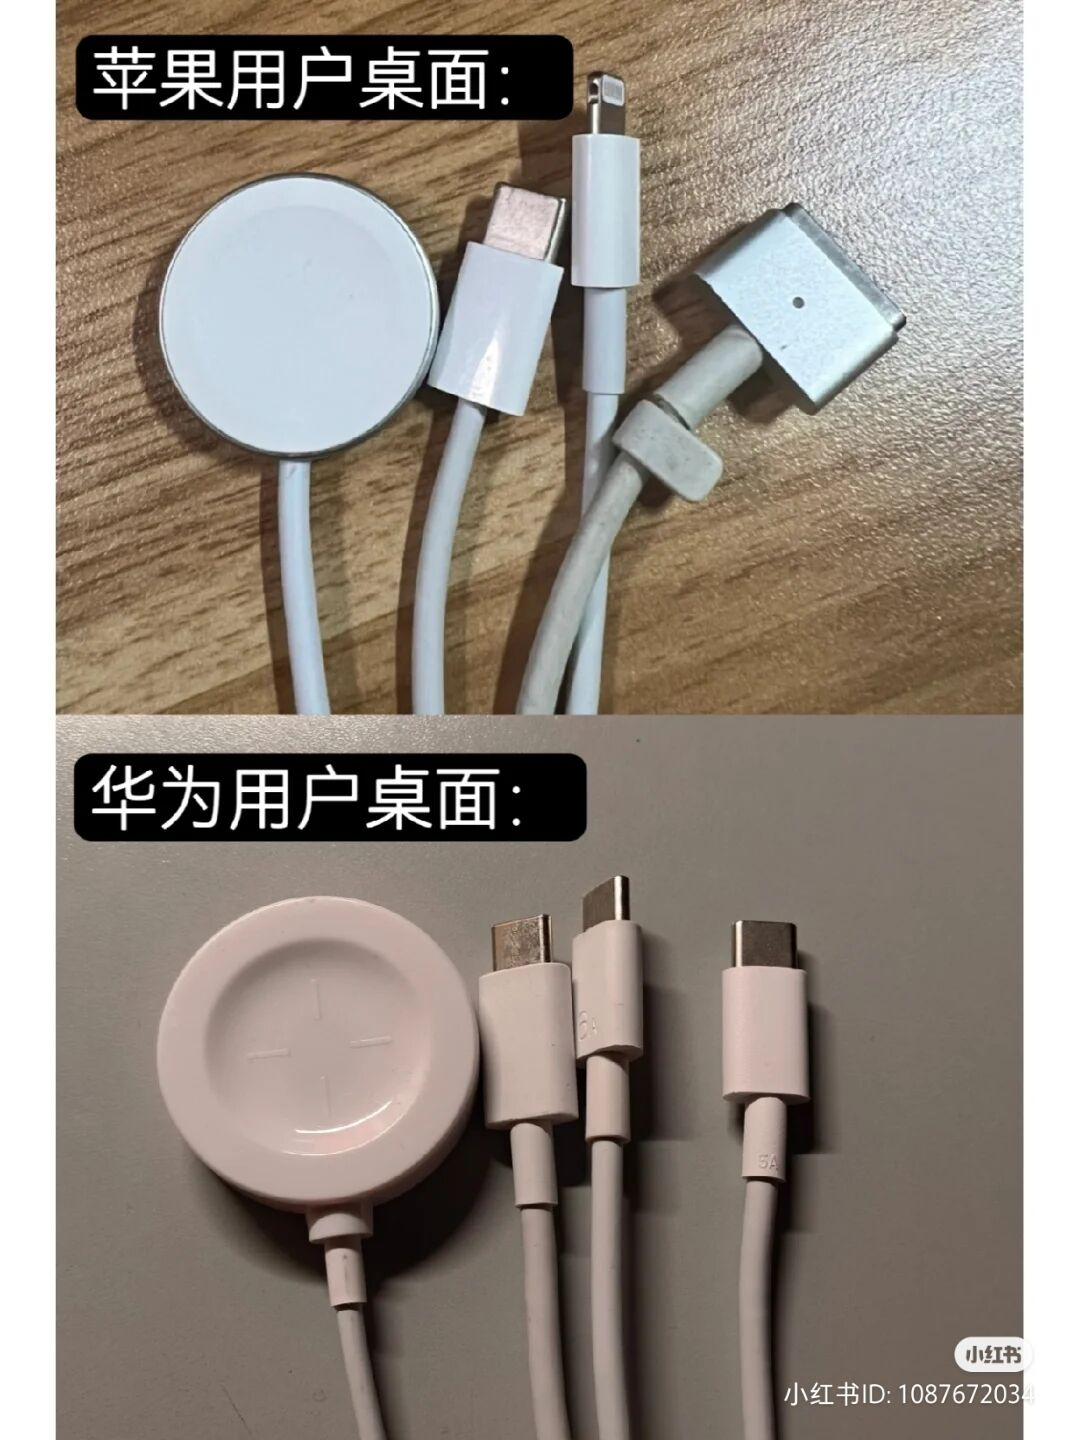
\includegraphics[scale=0.135]{figures/interface1.jpg}
        \end{minipage}
        \begin{minipage}{0.48\textwidth}
            \centering
            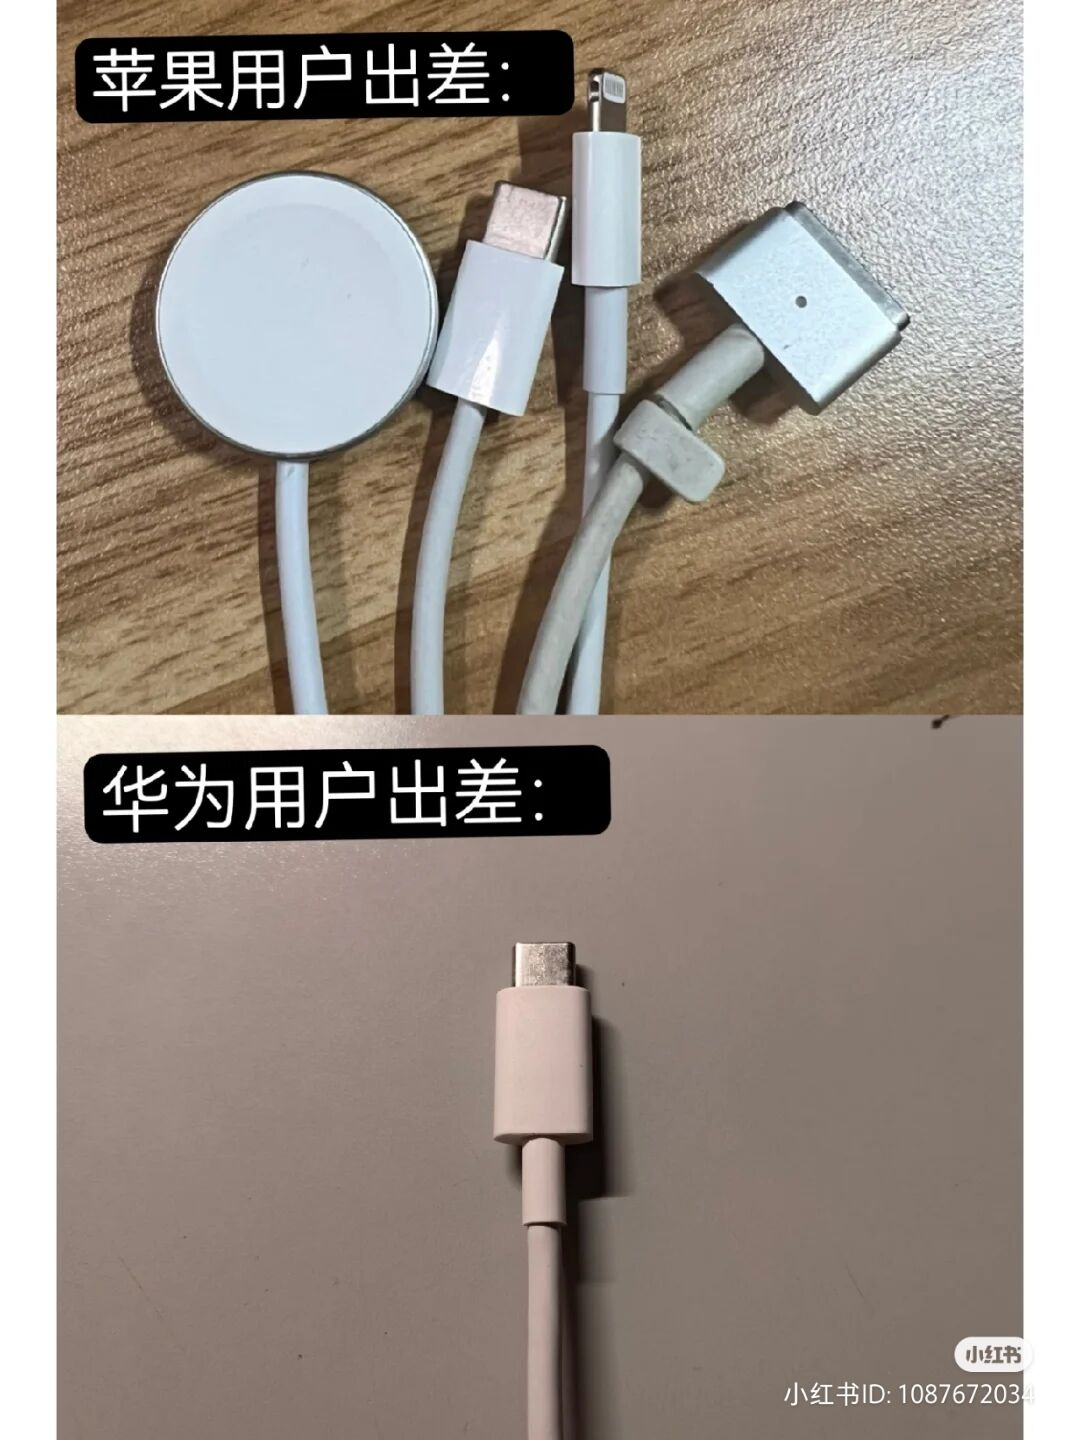
\includegraphics[scale=0.135]{figures/interface2.jpg}
        \end{minipage}
    \end{figure}
\end{frame}

\begin{frame}[fragile]{Using Iterators}
    \begin{cpp}
std::vector<int> v = {2, 3, 5, 7, 11, 13};
for (auto it = v.begin(); it != v.end(); ++it)
  *it = *it * *it;
for (auto it = v.begin(); it != v.end(); ++it)
  std::cout << *it << " ";
std::cout << std::endl;
    \end{cpp}
    \begin{itemize}
        \item The type of `\ttt{it}' is \ttt{std::vector<int>::iterator}.
        \item \ttt{v.begin()} returns the iterator pointing to the first element.
        \item \ttt{v.end()} returns the \textbf{off-the-end} iterator, positioned ``one past the end'' of the container.
        \item If the container is empty, we have \ttt{v.begin() == v.end()}.
    \end{itemize}
\end{frame}

\begin{frame}[fragile]{Iterator Operations}
    The iterator of every container supports these operations:
    \begin{center}
        \begin{tabular}{|ll|}
            \hline
            \begin{cpp}
*iter
            \end{cpp} & \footnotesize Returns reference to the element denoted by \ttt{iter}.\\
            \begin{cpp}
iter->mem
            \end{cpp} & \footnotesize Equivalent to \ttt{(*iter).mem}.\\
            \begin{cpp}
++iter
            \end{cpp} & \footnotesize Increments \ttt{iter} to refer to the next element in the container.\\
            \begin{cpp}
iter++
            \end{cpp} & \footnotesize Postfix version. Returns the copy of the original iterator.\\
            \begin{cpp}
==, !=
            \end{cpp} & \footnotesize Equal iff both iterators are pointing to the same position.\\
            \hline
        \end{tabular}
    \end{center}
    \begin{itemize}
        \item Dereferencing or incrementing an off-the-end iterator is undefined behavior.
    \end{itemize}
\end{frame}

\begin{frame}[fragile]{Examples}
    Count the number of upper-case letters and convert them to lower-case.
    \pause
    \begin{cpp}
int upper_cnt = 0;
for (auto it = s.begin(); it != s.end(); ++it) {
  if (std::isupper(*it)) {
    ++upper_cnt;
    *it = std::tolower(*it);
  }
}
    \end{cpp}
    \pause
    Convert the first word to upper-case.
    \pause
    \begin{cpp}
for (auto it = s.begin();
    it != s.end() && !std::isspace(*it); ++it)
  *it = std::toupper(*it);
    \end{cpp}
\end{frame}

\begin{frame}[fragile]{Range-\bluett{for}}
    The range-based \bluett{for} loop is treated as traversing using iterators.
    \begin{cpp}
for (auto x : v)
  do_something(x);
// Equivalent:
for (auto it = v.begin(); it != v.end(); ++it) {
  auto x = *it;
  do_something(x);
}
    \end{cpp}
\end{frame}

\begin{frame}[fragile]{Range-\bluett{for}}
    \begin{cpp}
for (const auto &x : v)
  do_something(x);
// Equivalent:
for (auto it = v.begin(); it != v.end(); ++it) {
  const auto &x = *it;
  do_something(x);
}
    \end{cpp}
    \pause
    \begin{itemize}
        \item Any object that could be traversed using the range-\bluett{for} loop must provide \ttt{begin()} and \ttt{end()}, which return an iterator that supports
        \begin{itemize}
            \item \bluett{operator*}: dereference
            \item \bluett{operator++}: prefix increment
            \item \bluett{operator!=}
        \end{itemize}
    \end{itemize}
\end{frame}

\begin{frame}[fragile]{\ttt{const\_iterator}}
    On a \const object, \ttt{begin()} and \ttt{end()} return a different iterator type:
    \begin{cpp}
inline void print_vector(const std::vector<int> &v) {
  for (auto it = v.begin(); it != v.end(); ++it)
    std::cout << *it << " ";
  std::cout << std::endl;
}
    \end{cpp}
    \begin{itemize}
        \item \ttt{it} here is of type \ttt{vector<int>::const\_iterator}.
        \item Dereferencing \ttt{it} returns a reference-to-\bluett{const}, which is not modifiable.
        \item Since C++11, we have explicit way to obtain \ttt{const\_iterator}s: The \ttt{cbegin()} and \ttt{cend()} member functions.
    \end{itemize}
\end{frame}

\begin{frame}[fragile]{Other Iterator Operations}
    Operations Supported by \ttt{vector} and \ttt{string} iterators:
    \begin{center}
        \begin{tabular}{|ll|}
            \hline
            \begin{cpp}
iter + n
            \end{cpp} & \footnotesize Returns an iterator positioned \ttt{n} elements forward.\\
            \begin{cpp}
iter - n
            \end{cpp} & \footnotesize Returns an iterator positioned \ttt{n} elements backward.\\
            \begin{cpp}
n + iter
            \end{cpp} & \footnotesize Equivalent to \ttt{iter + n}.\\
            \begin{cpp}
iter += n
            \end{cpp} & \footnotesize Equivalent to \ttt{iter = iter + n}.\\
            \begin{cpp}
iter -= n
            \end{cpp} & \footnotesize Equivalent to \ttt{iter = iter - n}.\\
            \begin{cpp}
iter1 - iter2
            \end{cpp} & \footnotesize Returns the distance between two iterators.\\
            \begin{cpp}
<,<=,>,>=
            \end{cpp} & \footnotesize Relational operators.\\
            \hline
        \end{tabular}
    \end{center}
    \begin{itemize}
        \item The return-type of \ttt{iter1 - iter2} is a \textbf{type-alias member} named \ttt{difference\_type}. e.g. \ttt{string::difference\_type}. It is a signed integer type.
        \item \ttt{iter1 - iter2} returns the number that when added to \ttt{iter2} yields \ttt{iter1}.
    \end{itemize}
\end{frame}

\begin{frame}[fragile]{Relational Operators of Iterators}
    \ttt{<, <=, >, >=}: comparing the positions of two iterators in the container.
    \begin{itemize}
        \item If they are not positioned in the same container, the result is undefined.
        \item Why did I always use \ttt{!=} in the \bluett{for} loops?
        \pause
        \begin{itemize}
            \item Not all kinds of iterators support \ttt{<, <=, >, >=}, but all of them support \ttt{==} and \ttt{!=}.
        \end{itemize}
    \end{itemize}
\end{frame}

\end{document}